\section{Codes}

\begin{definition}
Discrete Memoryless Source (DMS) 离散无记忆信源 \\
1. 压缩后有唯一解码 \\
2. 无损压缩 \\
3. 压缩后用尽可能少的比特表示
\end{definition}

Let $c(x)$ denote the codeword for $x$, $l(x)$ denote the length of $c(x)$, $p_X(x)$ denote the probability of $x$.

假设所有的符号 $X_i\stackrel{i.i.d.}{\sim}p_X(x)$, 则平均码长为
$$\mathbb{E}[L]=\overline{L}=\sum_{x}p_X(x)l(x)$$

\begin{figure}[htbp]
    \centering
    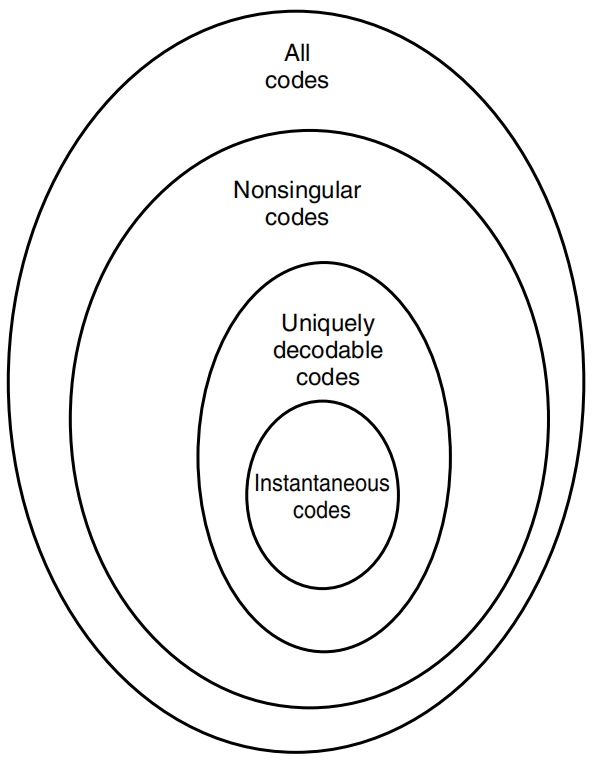
\includegraphics[width=0.4\textwidth]{./figures/chapter3/codes.png}
\end{figure}
Classes of codes:
\begin{itemize}
\item[1.] Nonsingular codes: 无歧义解码
$$x\neq x'\Rightarrow c(x)\neq c(x')$$
\item[2.] uniquely decodable codes: 有唯一解码
\item[3.] Instantaneous codes / Prefix codes(前缀码): 无 comma 可以及时解码 \\
e.g. codebook=$\{11,110\}$, 解码时遇到"11"无法及时解码
\item[4.] Fixed length codes: 定长码 \\
Alphabet size: $M$, code length: $L$, 则 $2^L\geq M$以表示所有的符号, i.e.
$$L=\lceil\log M\rceil\Rightarrow \log M\leq L < \log M+1$$
Code-blocking: 将$n$个symbol组合成一个block
\begin{figure}[htbp]
    \centering
    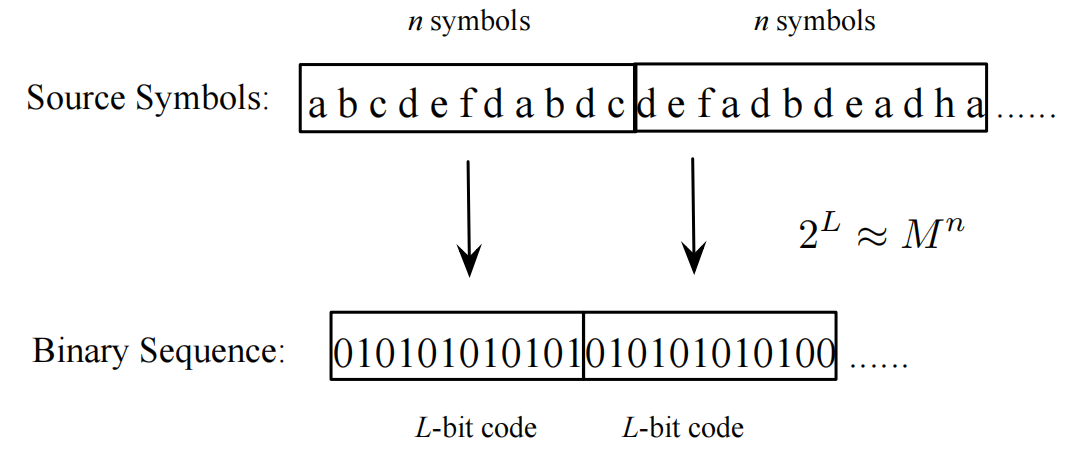
\includegraphics[width=\textwidth]{./figures/chapter3/code_blocking.png}
\end{figure}
$$L=\lceil\log M^n\rceil,\overline{L}=\dfrac{L}{n}\Rightarrow \log M\leq L < \log M+\dfrac{1}{n}$$
当$n$足够大是, 保证平均码长最优$\overline{L}\to\log M$, 但是空间(码本大小)指数级增加: $M^n$.\\
\textbf{定长码都是非前缀码!}

\item[5.] Variable length codes: 变长码 \\
无 comma 时可能会有歧义(非前缀码可以避免).
\end{itemize}